%!TEX ROOT = ../mainCZ.tex
%\input{./1_text/3_mat_a_met/2}

Tuto část uživatlského manuálu je nutné považovat za spíše teoretickou, popisující jednotlivé výpočetní vztahy, které jsou v modelu využity. V případě, že to lépe popisuje zvolené řešení jsou zde uvedeny i popis příslušné části zdrojového kódu.


\subsection{Použité vztahy a jejich odvození} \label{modelovani}


%	\subsubsection{Použité rovnice}
	%%!TEX ROOT = ../mainCZ.tex
% 
% 
% 
%
% Plošný povrchový odtok
%
%
%

\section{Bilanční rovnice} 

% 
Základním řešeným vztahem je aktuální bilance celkového zásoby
\begin{equation}
\acs{dS} = \acs{Itot} - \acs{Otot},
\label{eq:bilobecne}
\end{equation}
% 
% 
% 
% kde se aktuální změna  zásoby $S$ rovná rozdílu sumy aktuálních přítoků  \acs{Itot} a sumy aktuálních odtoků \acs{Otot}.
\begin{tabular}{rrl}
  kde \jj{dS}{,}
      \jj{Itot}{,}
      \jj{Otot}{.}
\end{tabular}


Podle složek povrchového odtoku a dalších procesů lze \acs{Itot} a \acs{Otot} v rovnici~(\ref{eq:bilobecne}) dále rozepsat na
$$
  \acs{Itot} = \acs{ES} + \acs{Oin},
$$
$$
  \acs{Otot} = \acs{Inf} + \acs{Oout},
$$
% 
% kde \acs{Oin} je přítok ze sousední výpočetní buňky (buněk) a \acs{Oout} je odtok z dané buňky. 
\begin{tabular}{rrl}
  kde \jj{Oin}{,}
      \jj{Oout}{,}
      \jj{ES}{,}      
      \jj{Inf}{.}
\end{tabular}


Bilanční rovnici pro buňku $i$ v čase $t$ lze rozepsat jako:




\begin{equation} 
\frac{\mathrm{d}S}{\mathrm{d}t} = \acs{ES}_{i,t-1} + \sum_j^m \acs{Oin}_{j,t-1} - \acs{Inf}_{i,t-1} - \acs{Oout}_{i,t-1},
\label{eq:bilancnirceV}
\end{equation}
% 
% 
% 
% kde $m$ jsou buňky, odkud vtéká voda do buňky $i$. 
\begin{tabular}{rrl}
  kde & $m$ & jsou buňky, z nichž vtéká voda do buňky $i$. 
\end{tabular}


V aktuální verzi modelu \smod se $m$ řídí pomocí jednosměrného odtokového algoritmu \acs{D8}.
% se liší podle použitého odtokového algoritmu jednosměrného \acs{D8} nebo vícesměrného \acs{mfda} ({\it multi-flow direction algorithm}) \pozn{ citace}. 
Model \smod řeší časový krok explicitně, veličiny v čase $t-1$ na pravé straně rovnice (\ref{eq:bilancnirceV}) jsou při řešení času $t$ známé.
% Objem srážky \acs{ES} a infiltrované množství \acs{Inf} lze určit přímo při výpočtu časového kroku $t$. Přiteklé a odteklé množství vody \acs{Oin} a \acs{Oout} z časového kroku $t-1$ (což odpovídá explicitnímu řešení časové derivace). 




Při samotném řešení se v modelu \smod operuje s veličinami ve výškových jednotkách ($m$) a intenzitách ($m/s$). Pokud celou rovnici~(\ref{eq:bilancnirceV}) vydělíme velkostí buňky \acs{bunka} a vyjádříme časovou derivaci jako diferenci ($\frac{\mathrm{d}\acs{hsur}_{i,t}}{\mathrm{d}t} \approx \frac{\acs{hsur}_{i,t} - \acs{hsur}_{i,t-1}}{\acs{dT}}$), vypadá rovnice~(\ref{eq:bilancnirceV}) následovně:

%nejsou to náhodou objemové jednoty, které dělíme plochou

\begin{equation} 
\acs{hsur}_{i,t} = \acs{hsur}_{i,t-1} + \acs{dT}\left(\acs{es}_{i,t-1} + \sum_j^m \acs{oin}_{j,t-1} - \acs{inf}_{i,t-1} - \acs{oout}_{i,t-1}\right),
\label{eq:bilancnirce}
\end{equation}
% 
% 
% 
% 
% kde \acs{hsur} je výška hladiny na povrchu, \acs{es} je intenzita srářky, \acs{inf} je intenzita infiltrace, \acs{oin}(\acs{oout}) odteklá (přiteklá) výška za čas. 
\begin{tabular}{rrl}
  kde \jj{hsur}{,}
      \jj{es}{,}
      \jj{inf}{,}
      \jj{oin}{,}
      \jj{oout}{.}
\end{tabular}
% 
% 


V následujícím textu jsou popsány jednotlivé členy za pravé straně rovnice~(\ref{eq:bilancnirce}).


% 
% 
% 
% 
% 
% 
% Efektivní srážka \acs{ES}
% 
% 
% 
% 
% 
% 
% 
\subsection{Efektivní srážka \acs{es}} 

Srážka je příčinou celého erozního procesu. Vzhledem k tomu, že je \smod epizodní model zadává se srážka v podobě konkrétní nebo návrhové srážky, která začíná s prvním časovým krokem výpočtu. Model počítá s vlivem intercepce, tedy že určitá část srážky bude zachycena rostlinami díky jejich potenciální intercepci \acs{PotI}. Míra zachycení v každém časovém kroku (\acs{dT}) výpočtu je definována  pomocí poměrné plochy listové \acs{Lai} (například \pozn{ citace}).

Označme množství srážky, které dopadá na povrch půdy i rostliny během \acs{dT} potenciální srážkou \acs{PS}. Část \acs{PS}, která zůstane  na povrchu rostliny během časovém kroku \acs{dT}, se dá vyjádřit jako násobek srážky \acs{PS} a \acs{Lai},
$$
\acs{PS}\ I_{LAI}.
$$
% 
Z tohoto vztahu vyplývá, že množství, které propadne povrchem listů, je 
$$
\acs{PS}(1 - I_{LAI}).
$$

Potenciální intercepce \acs{PotI} se začne plnit na začátku srážkové epizody. Výsledná intenzita efektivní srážky v čase $t$ je pak určena jako

$$
   \acs{es}_t= 
    \begin{cases}
     \acs{PS}_t(1 - I_{LAI}),& \text{pokud} \sum_{\bar{t} = t_{init}}^{t} (\acs{PS}_{\bar{t}}\ I_{LAI}) <= \acs{PotI}\\
     \acs{PS}_t,             & \text{jinak}
   \end{cases}
$$


% $$
%  \acs{es}_t = MAX(0;\sum_{\bar{t} = t_{init}}^{t}\left(\acs{PS}_{\bar{t}}(1 - I_{LAI})\right)-\acs{PotI}))/\acs{dT},
% $$
% kde suma $\sum_{\bar{t} = t_{init}}^{t}$ vyjadřuje množství srážky které propadlo povrchem listů plodiny od počátečního času $t_{init}$ do času $t$.
\begin{tabular}{rrl}
  kde \jj{PS}{,}
      \jj{Lai}{,}
      \jj{PotI}{\ a}
      & $\sum_{\bar{t} = t_{init}}^{t} (\acs{PS}_{\bar{t}}\ I_{LAI}) $ & vyjadřuje množství srážky, které propadlo \\
      && povrchem listů plodiny od počátečního času $t_{init}$ do času $t$.
      \label{srazka}
\end{tabular}



% 
% 
% 
% 
% 
% 
% 
% 
% 
% 
\subsection{Intenzita infiltrace \acs{inf}}

V modelu je použita infiltrace podle Philipa \citep{philip1957} v~následujícím tvaru (pro příslušnou buňku $i$):
\begin{eqnarray} \label{eq:phillip}
\acs{inf} = \frac{1}{2}\acs{Sorb}t^{-1/2}+\acs{Ks}.
\end{eqnarray}
% 
% 
\begin{tabular}{rrl}
  kde \jj{inf}{,}
      \jj{Sorb}{\ a}
      \jj{Ks}{.}
\end{tabular}




Philipova infiltrační rovnice byla zvolena především z důvodu relativně malého počtu vstupních parametrů. Tato zjednodušená rovnice má dva členy: nasycenou hydraulickou vodivost \acs{Ks} a sorptivita \acs{Sorb}. Autoři modelu si byli vědomi omezení použití Philipovy rovnice vyplývající z podmínek, za kterých byla odvozena.  Možné odchylky způsobené volbou této rovnice odpovídají odchylkám v heterogenitě půdy a kvalitě ostatních vstupů, na jejichž základě model pracuje. Čas $t$ ve vztahu~(\ref{eq:phillip}) je čas od začátku srážky, který by měl být v epizodním modelu totožný s počátečním časem výpočtu. Tato nezbytná podmínka by měla být brána v potaz při přípravě vstupních dat. 
% 
% 
% 
% 
% 
% 
% 
% 
% 
% 
% 
\section{Povrchový odtok  \acs{oin}, \acs{oout}} \label{sec:povrch_odtok}


V modelu jsou uvažovány dvě složky povrchového odtoku: \textbf{plošný povrchový odtok} a \textbf{soustředěný odtok v rýhách}. Soustředěný odtok v rýhách je ve \smod řešen explicitně. Vznik soustředěného odtoku je podmíněn překročením limitní rychlosti, resp. limitního tečného napětí (viz kapitola \ref{sec:soustredenyodtok}).

\subsection{Plošný povrchový odtok} \label{sec:plosny_odtok}

Rovnice plošného odtoku vychází z použití teorie kinematické vlny při řešení pohybové rovnice Saint-Venantových (SV) rovnic. Použití toho přístupu předpokládá mělké povrchové proudění po dlouhém plochém\footnote{Plochém ve smyslu ne příliš zakřiveném. Nejedná se tedy o hladký povrch.} povrchu. Za těchto podmínek lze u pohybové rovnice SV rovnic zanedbat lokální změny kinetické a potenciální energie a lokální zrychlení. Při tomto zjednodušení lze řešit povrchový tok jako ustálené proudění~\citep{miller1984basic}. Plošný povrchový odtok pak lze řešit pomocí obecného mocninného vztahu \pozn{v anglicke literature tomu rikaj power law, tak nevim jak cesky} jako
% 
% 
% 
\begin{equation}
  \acs{qsur} = \acs{a}\acs{hsur}^{\acs{b}},
  \label{eq:plos_prutok}
\end{equation}
% 
% 
% 
\begin{tabular}{rrl}
  kde \jj{qsur}{,}
      \jj{a}{\ a}
      \jj{b}{.}
\end{tabular}\\
Parametr \acs{a} je řešený podle vztahu:
$$
a = \acs{X}\acs{I}^{\acs{Y}},
$$
\begin{tabular}{rrl}
  kde \jj{X}{,}
      \jj{Y}{\ a}
      \jj{I}{.}
\end{tabular}

Parametry \acs{a} a \acs{b} respektive \acs{X} a \acs{Y} jsou odvozeny na základě měření \citep{Neumann15:232823}, jejich hodnoty pro různé půdní typy jsou ukázány v tabulce~\ref{tab:Neuman_param} v příloze~\ref{sec:priloha}. Z vyhodnocení vyplývá, že parametr \acs{b} je závislý pouze na půdním druhu. Parametr \acs{a} je závislý nejen na půdním druhu, ale také na sklonu svahu $I$. Pokud je na povrchu půdy pokryt vegetací, je třeba provést korekci pomocí Manningova součinitele drsnosti pro povrchoví odtok. Parametr \acs{a} je pak definován jako
$$
  a = \frac{\acs{X}\acs{I}^{\acs{Y}}}{100\acs{n}},
$$
\begin{tabular}{rrl}
  kde \jj{n}{.}
\end{tabular}



Odteklá resp. přiteklá výška je pak dopočítána jako
$$
   \acs{oout} (resp.\ \acs{oin}) = \frac{\acs{effVrst}}{\acs{bunka}}\acs{qsur}
$$
%
% 
\begin{tabular}{rrl}
  kde \jj{effVrst}{\ a}
      \jj{bunka}{.}
\end{tabular}

Efektivní vrstevnice \acs {effVrst} je největší délka v buňce rastru kolmou na směr odtoku. Jedná se tedy o délku průmětu průtočné plochy na danou buňku.

% $$
% q_{sur} [m^{3}/s] = Ah_{sur}^{b} \Rightarrow \frac {1}{n} a h_{sur}^{X} i_{0}^{Y}
% $$


% 
% 
% 
% 
% 
% 
% 
% 
% 
% 
% 

\subsubsection{Odvozené veličiny}

Z vypočteného specifického průtoku, velikosti řešeného elementu a délky časového kroku lze dopočítat objem odtoku:
$$
  \acs{Vout} = \acs{dT}\ \acs{effVrst}\acs{qsur},
$$
% 
% 
% 
% 
\begin{tabular}{rrl}
  kde \jj{Vout}{.}
\end{tabular}


Pro posouzení erozního ohrožení a pro určení vzniku rýhy je v každé buňce vypočítávána rychlost proudění a tečné napětí. Za předpokladu, že se jedná a proudění vody o malé hloubce, lze rychlost proudění odvodit ze specifického průtoku a výšky hladiny:
% 
% 
% 
% 
% 
\begin{equation}
  \acs{vsur} =  \frac{\acs{qsur}}{\acs{hsur}},
  \label{eq:v}
\end{equation}
% 
% 
% 
\begin{tabular}{rrl}
  kde \jj{vsur}{.}
\end{tabular}


\subsubsection{Určení vzniku rýhy}\label{sec:vznikryhy}

Povrchový odtok způsobuje tření na povrch půdy. Za určitých podmínek je soudržnost půdy nižší než tečné napětí proudící vody na jejím povrchu. Je několik způsobů jak tento moment určit \pozn{citace}. V modelu \smod jsou implementovány dva způsoby odvození: překročením kritického tečného napětí a překročením nevymílací rychlosti. Z obou odvození je určena kritická výška hladiny \acs{hcrit} povrchového odtoku po jejímž překročení začne vznikat rýha. 

Vztah pro výpočet tečného napětí je v modelu \smod definován podle \cite{Schwab1993} jako
% 
% 
% 
\begin{equation}
\acs{tausur} = \acs{ro} \acs{g} \acs{hsur} \acs{I}\acs{K},
 \label{eq:tau}
\end{equation}
% 
% 
% 
\begin{tabular}{rrl}
  kde \jj{tausur}{,}
      \jj{ro}{,}
      \jj{g}{,}
      \jj{I}{\ a}
      \jj{K}{.}
\end{tabular}

Vznik rýh je také považován za limitní z hlediska erozní ohroženosti. Umístění prvků protierozní ochrany by mělo být vedeno tak, aby nedocházelo ke vzniku rýh. Kritické hodnoty nevymílacích rychlostí a tečných napětí jsou pro jednotlivé půdní druhy a druh vegetace \pozn{v tabulce na kterou to ma odkazovat je to jen pro pudni typ ne pro vegetaci} převzaty z předchozích verzí modelu (podle \cite{DyrovaE.1984}) a jsou uvedeny v tabulce.
\pozn{na toto tema jsem nasel v adr tab jen jednu tabulku, tam je citovan vrana, ale zase neni v zadnym *.bib}
V literatuře se setkáme i s odlišnými hodnotami. Například M. A. Velikanov stanovil kritickou nevymílací rychlost pro půdy 0.24 $m/s$   \pozn{divna citace typka s jinym jmenem}\citep{CabikJ.1963}, což je hodnota nižší, než kterou stanovila E. Dýrová.

Přepočet kritické nevymílací rychlost na kritickou výšku hladiny \acs{hcrit} je odvozen z rovnic (\ref{eq:plos_prutok}) a (\ref{eq:v}) jako
\begin{equation}
  \acs{hcrit} = \frac{100\ \acs{n}\ \acs{vcrit}^{1/(\acs{b}-1)}}{\acs{a}},
  \label{eq:hcrit_v}
\end{equation}
\begin{tabular}{rrl}
  kde \jj{hcrit}{\ a}
      \jj{vcrit}{.} 
%   
\end{tabular}


Výpočet kritické výšky hladiny z tečného napětí je jednoduše odvozen z vzorce (\ref{eq:tau}) jako
\begin{equation}
  \acs{hcrit} = \frac{\acs{taucrit}}{\acs{ro} \acs{g} \acs{I}},
  \label{eq:hcrit_tau}
\end{equation}

\begin{tabular}{rrl}
  kde \jj{taucrit}{.} 
%   
\end{tabular}


Pro každou buňku výpočetní oblasti je spočítáno \acs{hcrit} pomocí obou odvození (\ref{eq:hcrit_v}) a (\ref{eq:hcrit_tau}). Podmínka v modelu následné vybere menší z hodnot, která je pak pří výpočtu použita jako kritérium vzniku rýh \pozn{to chce asi strucne dovysvetlit proc bere tu mensi a doplnit literaturu}. 
kritická nevymílací rychlost a kritické tečné napětí jsou vstupní parametry modelu. Návrh hodnot pro model \smod je ukázán v tabulce~\ref{tab:kriticke} v příloze~\ref{sec:priloha}. 



% 
% 
% 
% 
% 
% 
% 
% 
% 
% 
% 
\subsection{Soustředěný odtok v rýhách} \label{sec:soustredenyodtok}

Výpočet soustředěného odtoku v rýhách implementovaný v modelu SMODERP vychází z několika předpokladů:
\begin{enumerate}
  \item Zavedení stejných zjednodušujících předpokladů výpočtu proudění jako v~případě výpočtu plošného povrchového odtoku (teorie kinematické vlny). Předpokladem je, že se tok ve všech časech a ve všech buňkách vždy dostane do ustáleného, tady že se vždy jedná o ustálené proudění. Při ustáleném proudění se předpokládá sklon \pozn{nebo to byt sklon treci síly?} dna \acs{I} paralelní se sklonem hladiny vody v rýze a neměnná drsnost v celé délce buňky. Průtok v rýze je tedy vyjádřen pomocí Chézyho rovnice v Mannigově tvaru:
  \begin{equation}
    \acs{qrill} = \acs{vrill} \acs{A} = \acs{A} \frac{1}{\acs{n}} \acs{Rrill}^{2/3} \acs{I}^{1/2}  ,
    \label{eq:qrill}
  \end{equation}
  \begin{tabular}{rrl}
    kde \jj{qrill}{,}
        \jj{vrill}{,}
        \jj{A}{,}
        \jj{n}{\ a}
        \jj{Rrill}{.}
  \end{tabular}

  
  
  \item Soustředěný odtok vzniká v buňkách, kde dojde k překročení kritické výšky hladiny \acs{hcrit} (viz \ref{sec:vznikryhy}). Tato hodnota je určena pro každou buňku zvlášť na základě  hodnot kritického tečného napětí nebo kritické nevymílací rychlostí podle vzorců (\ref{eq:hcrit_v}) a (\ref{eq:hcrit_tau}).
  
  
  \item V každé buňce výpočetní oblasti může vzniknout pouze jedna přímá rýha bez ohledu na velikost kroku prostorové diskretizace. 
  
  
  \item Objem vzniklé rýhy odpovídá nadkritickému objemu vody \acs{Vrill}, který vychází ze vztahu:
  $$
  \acs{Vrill}= \acs{Vtot} - \acs{Vcrit} = MAX(0;\acs{hsur} - \acs{hcrit}) \acs{bunka}
  $$
  \begin{tabular}{rrl}
    kde \jj{Vrill}{,}
        \jj{Vtot}{,}
        \jj{Vcrit}{\ a}
        \jj{hcrit}{.}
  \end{tabular}
  

  \item Tvar přísného profilu rýhy je reprezentován obdélníkem, s pevným poměrem stran \acs{rratio}=výška/šířka rýhy. Velikost rýhy se zvětšuje pokud je nadkritické množství \acs{Vrill} větší než objem samotné rýhy, tak aby byl splněn předpoklad v předchozím bodě. Při zvětšovaná rýhy se tedy výška rýhy rovná výšce vodní hladiny v rýze (vlevo na obrázku~\ref{fig:rill_schema}). Pokud začne být nadkritické množství \acs{Vrill} menší než je objem rýhy a dochází k prázdnění rýhy. Velikost rýhy zůstává konstantní a rýze dochází pouze k poklesu hladiny (vpravo na obrázku~\ref{fig:rill_schema}). Hydraulický poloměr rýhy, která se zvětšuje nebo je konstantní, lze určit podle následujícího vztahu:
%  
% 
% 
%   Rozměry rýhy nejsou známy, protože rozměr rýhy \acs{hrill}, \acs{brill} se dynamicky mění v závislosti na množství vody během simulace. 
%   
  \begin{figure}
    \centering
    \includegraphics[width=0.9\textwidth]{./img/rill_schema.png}
    \caption{Příčný řez rýhy a výška vodní hladiny při plnění rýhy či ustálení proudění (napravo), tvar rýhy při jejím prázdnění (nalevo)}
    \label{fig:rill_schema}
  \end{figure}
% 
%   
  $$ 
    \acs{Rrill} = \frac{\acs{A}}{\acs{O}} = \dfrac{\acs{hrill} \acs{brill}}{\acs{brill}+2\acs{hrill}} \qquad kde \quad \acs{brill} = \dfrac{\acs{hcrit}}{\acs{rratio}}
  $$
  \begin{tabular}{rrl}
    kde \jj{brill}{,}
        \jj{O}{\ a}
        \jj{rratio}{.}
  \end{tabular}
  
  Hydraulický poloměr rýhy, ve které výška hladina oproti výšce rýhy klesá, se určuje jako 
  
  $$ 
    \acs{Rrill} = \frac{\acs{A}}{\acs{O}} = \dfrac{\acs{hrill} \acs{brill}}{\acs{brill}+2\acs{hrill}} \qquad kde \quad \acs{brill} = \dfrac{y}{\acs{rratio}}.
  $$
  
  
\end{enumerate}


% Pro výpočet průtoku v rýze \acs{qrill} je pak možné využít Chézyho rovnici v manningově tvaru:.

  Výška odtoku (resp. vtoku) z rýhy je vypočtena podle vzorce
  $$
    \acs{oinrill} (resp.\ \acs{ooutrill}) = \frac{\acs{qrill}}{\acs{brill}\acs{lrill}}.
  $$
  \begin{tabular}{rrl}
    kde \jj{lrill}{.}
  \end{tabular}

\subsection{Celková bilance}
Pokud dojde k vzniku rýh, je rovnice celkové bilance~(\ref{eq:bilancnirce}) rozšířena o členy vyjadřující soustředěný rýhový odtok a přítok z rýh sousedních buněk takto

\begin{equation} 
\acs{hsur}_{i,t} = \acs{hsur}_{i,t-1} + \acs{dT}\left(\acs{es}_{i,t-1} + \sum_j^m \acs{oin}_{j,t-1} - \acs{inf}_{i,t-1} - \acs{oout}_{i,t-1}  + \sum_k^n \acs{oinrill}_{k,t-1} - \acs{ooutrill}_{i,t-1} \right),
\label{eq:bilancnircerill}
\end{equation}
  \begin{tabular}{rrl}
    kde \jj{oinrill}{\ a}
        \jj{ooutrill}{.}
        & $n$ & jsou buňky, odkud vtéká voda z rýh do buňky $i$.
  \end{tabular}\\
 $n$ může být prázdná množina pokud není překročena kritická výška nebo no může rovnat $m$ z rovnice~\ref{eq:bilancnirce} pokud je použit odtokový algoritmus \acs{D8} a na všech sousedních buňkách buňky $i$ je překročena kritická výška hladiny. 





% Množství odtoku \acs{Orill} za \acs{dT} je pak možné stanovit podle vztahu:
% \begin{eqnarray}
% O_{rill_{i,t}} [m^{3}] = \Delta t q_{sur}
% \end{eqnarray}
% 
% Tvar bilanční rovnice \ref{bilancnirce} při zavedení odtoku v rýhách pak přechází na tvar:
% \begin{eqnarray}
%   H_{i,j,t} = H_{i,j,t-1} + ES_{i,j,t} + \sum\limits_{(i,j)\in M} O_{M_{t-1}} - O_{i,j,t} - I_{nf_{i,j,t}} \label{eq:bilancenew}
% \end{eqnarray}
% \begin{equation*}
%  M = \{ (k,l) | i-1 \leq k \leq i+1 ; j-1 \leq l \leq j+1 \}
% \end{equation*}



% \textit{kde $ O_{M} $ obecně znamená jak přítok plošný, tak soustředěný v rýhách, $ O $ celkový odtok, který se podle konkrétního stavu dělí na plošný a soustředěný}





\subsection{Poznámka nebo to dát do diskuse k článku} 
\begin{itemize}
\item Výsledný tvar blíží Maningově rovnici
\begin{eqnarray}
Q =\frac A {1}{n} R_{h}^{2/3} S^{1/2}
\end{eqnarray}
\item Přesněji pro tvar této rovnice pro plošný odtok, kdy se předpokládá proudění vody  o malé hloubce a tvar koryta je nahrazen jeho šířkou. Rovnice má pak tvar:
\begin{eqnarray}
Q =\frac {1}{n} h^{2/3} S^{1/2}
\end{eqnarray}
\item Že může být jiná rce infiltrace.
\item tvar rýhy - výzkum funkce?
\item jen jedna přímá rýha
\end{itemize}

%newb = math.sqrt(V/(rillRatio*l)) #KAvka, tohl eje divně
\section{Odtok hydrografickou sítí} \label{sec:tokyodtok}


\smod je zamýšlen také jako nástroj pro navrhování opatření v ploše povodí. Cílem je simulovat a navrhovat odtoky i v dočasné hydrografické síti, která je tvořena přirozeným nebo častěji umělým přerušením přirozené odtokové dráhy. Nejčastěji se jedná o příkopy a průlehy, které mají odváděcí a často protierozní funkci. 
Všechny prvky (síť vodních toků, příkopy, průlehy, atp.) jsou zadávány v rámci jednoho shapefile. Každý jednotlivý úsek je zadán jako konkrétní linie (feature). Výpočetně model pracuje v rastrové síti. V případě, že se na dané buňce rastru vyskytuje úsek hydrografické sítě, je voda dále odváděna tímto úsekem ve směru jeho sklonu  bez ohledu na směr plošného či soustředěného odtoku.


Proudění v těchto otevřených korytech je řešeno Mannigovou rovnicí ve tvaru:

\begin{equation}
    \acs{qstream} = \acs{A} \frac{1}{\acs{n}} \acs{Rstream}^{2/3} \acs{I}^{1/2}  ,
    \label{eq:qtok}
\end{equation}

% 
\begin{tabular}{rrl}
   kde \jj{qstream}{,}
       \jj{A}{,}
       \jj{n}{\ a}
       \jj{Rstream}{.}
\end{tabular}
  

Pro vlastní výpočet je třeba zadat typ a příčný profil daného prvku. Délka úseku a sklonu jsou převzaty z liniové vrstvy a z digitálního modelu terénu. Protože je model určen pro malá povodí jsou v modelu předpokládány pouze základní tvary příčných profilů (trojúhelník, obdélník, lichoběžník, parabola). Vzorce pro výpočet odtoku různými geometriemi jsou ukázany v příloze \ref{sec:priloha} v tabulce na obrázku~\ref{fig:tvary_koryt}. Model \smod je schopen řešit odtok liniovými prvky, které se zapojí do odtoku až při tvorbě povrchového odtoku i~odtok vodními toky se základním odtokem. Princip zadávání geometrie úseků hydrografické sítě je popsán v častí~\ref{cast:2} v kapitole~\ref{sec:vodnitoky} tohoto manuálu. 
  
Objem vody, který teže mezi jednolivýli úseky hydraulické sítě je určen jednoduše jako
$$
  V_{stream,out} = \acs{dT}\acs{qstream}.
$$





\pozn{ Tímto způsobem jsou zadány tvary prvků, které se v řešené lokalitě vyskytují.
\textbf{sem dát obrázek těch profilů}}


\pozn{\textbf{doplnit text jak probíhá vlastní výpočet} - tzn jak na sebe navazují jednotlivé úseky . a dát semka asi i nějaké  obrázky, jak to funguje. Je to v nějaké DP tuším (to najdu PK)}





\subsection{SMODERP 2D - postup výpočtu} \label{vypocet}
Tato verze modelu SMODERP je napsána v programovacím jazyce Python. V rámci kódu jsou od sebe oddělena část přípravy dat a samotné zpracování.
Příprava dat využívá v současné době nástroje z knihoven ArcGIS proto byl zvolen jako programovací jazyk Python, který je pro prostředí ArcGIS nativním programovacím jazykem. Proces samotného výpočtu již využívá pouze standardní knihovny Python, jako je knihovna \texttt{numpy}, nebo \texttt{math}, atp. Pro přehlednost je text rozdělen do třech částí, vstupní data \ref{kap:vstupy}, tok programu \ref{kap:tok} a výstupy \ref{kap:vystupy}

	%\subsubsection{Princip výpočtu} \label{kap:principvypoctu}
%	\input{./1_text/3_mat_a_met/CZsmoderp_princip}
		
	
	\subsubsection{Vstupy do modelu} \label{kap:vstupy}
	%%!TEX ROOT = ../mainCZ.tex




Vstupní data modelu jsou ve třech formátech: rastrovém, vektorovém a textovém. Do modelu vstupují informace o topografii řešeného území, informace o typech půd a vegetaci, informace o srážce atd. Základní formát vektorových dat je formát shapefile. Tento vektorový formát byl vytvořen firmou ESRI, ale je zpracovatelný i jinými GIS softwary. Parametry modelu jsou uloženy v atributové tabulce pod specifickým názvem pole. 
% Shapefile popisuje prvky jako body, linie nebo polygony. Každý prvek má obvykle nějaký atribut, který ho popisuje jako v tomto případě jméno, či typ půdy. 
V následujícím text jsou popsány náležitosti vstupních dat. 
% 
% Model pracuje s následujícími vstupy
Přehled vstupů do modelu je ukázán v tabulce~\ref{tab:vstupy}.


Princip pouštění modelu \smod v programu ArcGIS je popsán na konci této kapitoly (sekce~\ref{sec:intoolbox}). 
% 





% 

% 
\begin{sidewaystable}
% \begin{table}[]
\centering
\caption{Tabulka s přehledem vstulních dat modelu}
\label{tab:vstupy}
\small{
% \begin{tabular}{p{4cm}lp{2cm}p{5cm}}
\begin{tabular}{p{0.15\textwidth}lp{0.10\textwidth}p{0.25\textwidth}l}
\hline
Název                              & Typ dat                                               & Povinný / volitelný & Poznámka                                                                                      & Popis kapitole                                                       \\ \hline \hline
digitální model terénu             & \cellcolor[HTML]{96FFFB}{\color[HTML]{000000} raster} & Povinný           & Touto vrstvou se řídí i prostorová diskretizace                                                 & \ref{sec:vstupdmt}                                          \\ \hline
prostorové rozložení půd           & \cellcolor[HTML]{FFC702}vektor - polygony             & Povinný           & Polygon mají v atributové tabulce idenfikátor typu půdy                                         & \ref{sec:vstuppuda}                                        \\ \hline
prostorové rozložení typu vegetace & \cellcolor[HTML]{FFC702}vektor- polygony              & Povinný           & polygon mají v atributové tabulce idenfikátor typu vegetace                                     & \ref{sec:vstupvegetace} a \ref{sec:upravatabulkyparametru}   \\ \hline
srážková data                      & .txt soubor                                           & Povinný           & kumulativne zadaná srážka                                                                       &        \ref{sec:vstupsrazka}                                \\ \hline
maximální časový krok              & reálné číslo                                          & Povinný           & podle délky a intenzity srážky; doporučuje se 30 - 60 sekund                                    &    \ref{sec:vstupkrok}                                      \\ \hline
výstupní adrešář                   & text                                                  & Povinný           & adresář pro uložení výsledků (při začátku výpoštu se adresář vyčistí!)                          &    \ref{sec:vstupadresar}                           \\ \hline
bodové výstupy hydrogramů          & \cellcolor[HTML]{FCFF2F}vektor - body                 & Volitelný         & Body, kde se výpíší výsledky. Pokud je ve stejné buňce jako bod úsek hydrografické sítě, vypíše veličony v příslušné linii    &   \ref{sec:vstupbody}           \\ \hline
typ výpočtu                        & text                                                  & Povinný           & Uživatel má na výběr: pouze plošní odtok, plošný i rýhový odtok, plošný rýhový odtok i odtok hydraografickou sítí             &  \ref{sec:vstupryhovy}          \\ \hline
volba výcesměrného odtoku          & \cellcolor[HTML]{9698ED}logická proměnná              & Povinný           & Výchozí je jednosměrný odtok. Uživatel může zvolit výceměrný odtok.                                                           &     \ref{sec:vstupvicesmerny}   \\ \hline
paramtry půdy a vegetace           & \cellcolor[HTML]{67FD9A}tabulka                       & Povinný           & Tabulka parametrů půdy a vegetace. Názvy sloupců mají definované označení. Hodnoty se spojí s vektorovými vrstvami.           &   \ref{sec:upravatabulkyparametru}\\ line
hydrografická síť                  & \cellcolor[HTML]{F8FF00}vektor - linie                & Volitelný         & Prostorové rozložení hydrografické sítě. Atributová tabulka obsahu identifikátor jednolivých linií hydrografické sítě.        & \ref{sec:vodnitoky}             \\ \hline
parametry hydrografické sítě       & \cellcolor[HTML]{67FD9A}tabulka                       & Volitelný         & Tabulka parametrů jednotlivých částí hydraografické sítě. Názvy sloupců mají definované označení. Hodnoty se spojí s jednotlivými liniemi hydrografické sítě. &  \ref{sec:vodnitoky}     \\ \hline
volba arcgis výstupů               & \cellcolor[HTML]{9698ED}logická proměnná              & Povinný           & Výchozí formát výstupních rasterů je proprietární formát ERSI. Uživatel může zvolit textorý formát ASCII jako formát výstupních rasterů.                      & --- \\ \hline
\end{tabular}
}
% \end{table}
\end{sidewaystable}
% \begin{itemize} \itemsep 0pt
% \item digitální model terénu
% \item shapefile půd
% \item shapefile využití území
% \item srážkový soubor
% \item časový krok výpočtu a celková doba simulace
% \item výstupní adresář
% \item bodová vrstva pro generování hydrogramů
% \item výstupní adresář
% \item typ výpočtu
% \item volba výcesměrného odtoku
% \item tabulka půd a vegetace a kód pro připojení
% \item shapefile hydrografické sítě
% \item tabulka vodních toků a kód pro připojení
% \item volitelné formy výstupů
% \end{itemize}


\pozn{
\textbf{Nutno dodělat}
\begin{itemize} \itemsep 0pt
\item upravit podle aktuálního stavu
\item upravit a zjednosušit tuto kapitolu
\item propojit s tabulkama co jsou jinde v textu
\item vložit sem tabulky parametrů výpočtu pokud nejsou jinde
\end{itemize}
}















\subsection{Digitální model terénu} \label{sec:vstupdmt} 

Rastr digitálního modelu terénu nebo také DMT, či anglicky DTM (Digital Terrain Model) je souvislý povrch území obvykle znázorňující morfologii určité části Země. DMT rastr je složen z jednotlivých buněk. Nejčastější formou jsou buňky čtvercové, ale mohou mít i jiný tvar. \pozn{smoderp dela jen ctverce, takze mozna zbytecna vedlejsi veta} Velikost buněk se liší v závislosti na velikosti zobrazovaného území. Pro účely modelu \smod by minimální velikost buněk měla být 2 metry, optimum je však 5 metrů a více. Důležitá je i celková rozloha rastru, tedy počet buněk. Model byl testován na rastrech o velikosti od několika málo tisíc buněk. DMT jednoho z testovacích, povodí Nučice, obsahuje přes 125 tisíc buněk. Příklad DMT dalšího testovacího povodí Býkovice je ukázán na obrázku~\ref{fig:bykovicedmt}.


\begin{figure}
  \centering
  \includegraphics[width=0.5\textwidth]{./img/DMT_byk.png}
  \caption{Výřez digitálního modelu terénu povodí Býkovice}
  \label{fig:bykovicedmt}
\end{figure}

 
 
 
 
 
 
 
 
 
 
 
 
 
 
 
 
 
 
 
\subsection{Půdní data} \label{sec:vstuppuda}

Datové zdroje vlastností půd jsou v rámci České Republiky roztříštěné. Model \smod pracuje s jednou vstupní vrstvou půd. Příprava této vrstvy z dostupných dat je otázkou preprocessingu a propojení relevantních zdrojů. V zásadě jsou tři základní dostupné datové zdroje půdních vlastností. Odděleně připravená \pozn{to: jinou metodou pripravene si nejsem jist} data na zemědělské a lesní půdě nebo bezešvá vrstva půd KPP odpovídající měřítku 1:200000.

V České Republice se na zemědělské půdě standardně využívá rozdělení podle Novákovi klasifikace. Půda je rozdělena podle obsahu tzv. jílových částic na půdy \cite{kavka} \pozn{ v bib/bib.bib zadna polozka s oznacenim kavka neni...}:
\begin{itemize} \itemsep -3pt
  \item písčité
  \item hlinitopísčité
  \item písčitohlinité
  \item hlinité
  \item jílovitohlinité
  \item jílovité
  \item jíl
\end{itemize}

Na lesních půdách je v České Republice standardně využíván popis kategorií podle klasifikace USDA.
Obrázek~\ref{fig:pripravapar_vyrez}b ukazuje výřez připravené vrstvy. Pro určení charakteristik je nutné, aby atributová tabulka dané vrstvy obsahoval identifikátor půdního typu. Identifikátor odkazuje na půdní charakteristiky, které jsou ale uložené ve zvláštní tabulce (viz níže). Mezi půdní charakteristiky a parametry používané modelem patří: \acs{HyVod} - \acl{HyVod}; \acs{Sorb} - \acl{Sorb}; \acs{n} - \acl{n},  \acs{a} - \acl{a}, \acs{b} - \acl{b}, \acs{X} - \acl{X} a  \acs{Y} - \acl{Y}. Hodnoty těchto parametrů jsou definované v tabulce v kapitole~\ref{sec:upravatabulkyparametru}. Fyzikální význam těchto parametrů a jejich implementace v modelu jsou popsány v části~\ref{cast:1} toho manuálu. 


% \begin{figure}
%   \centering
%   \includegraphics[width=0.5\textwidth]{./img/pudy.png}
%   \caption{výřez půdní mapy s vyznačenými půdními druhy}
%   \label{fig:bykovicepuda}
% \end{figure}
% 
%  
 
 
 
 
 
 
 
 
 
 
 
 
 
 
 
\subsection{Data o využití území} \label{sec:vstupvegetace}
\pozn{pk - doplnit zdroje takovych dat}
Obdobně jako u půdních dat je vstupem vektorový shapefile popisující využití území. Mezi základní typy, pro které byl model testován, patří:
\begin{itemize} \itemsep -3pt
  \item atropogení a zpevněné plochy  
  \item holá půda bez vegetace
  \item les
  \item sad
  \item travní porosty
  \item zemědělské plodiny širokořádkové\footnote{Širokořádkové plodiny jsou například brambory, kukuřice, řepa, sója a slunečnice.}
  \item zemědělské plodiny úzkořádkové\footnote{Úzkořádkové plodiny jsou obiloviny nebo řepka.}
\end{itemize}


Shapefile popisující využití území je ukázán na obrázku~\ref{fig:pripravapar_vyrez}c. Obdobně jako u půd v předchozí sekci je třeba atributovou tabulku tohoto shapefilu doplnit o identifikátor daného využití území. Tento identifikátor odkazuje na charakteristiky daného povrchu definované ve zvláštní tabulce (popsáno v sekci~\ref{sec:upravatabulkyparametru}). Parametry související s využitím území, které vstupující do modelu jsou zejména \acs{PotI} - \acl{PotI} a \acs{Lai} - \acl{Lai}. Jejich konkrétní použití je popsáno v části~\ref{cast:1} toho manuálu. 
% 
% \begin{figure}
%   \centering
%   \includegraphics[width=0.5\textwidth]{./img/LandCover.png}
%   \caption{Ukázka vektorové vrstvy využití území -  Land Cover}
%   \label{fig:bykovicevegetace}
% \end{figure}
% 
% 
% 















\subsection{Tabulka parametrů půdy a využití území}  \label{sec:upravatabulkyparametru}

Další povinný vstup je tabulka, která obsahuje hodnoty jednotlivých parametrů popsaných v předešlých kapitolách a části~\ref{cast:1} toho manuálu. Na tuto tabulku se odkazují identifikátory půdního typu a typu využití území definované jako pro jednotlivé polygony. Tato tabulka může být do modelu vlože jako textový soubor. Na obrázku~\ref{fig:pripravapar_vyrez}e je ukázán příklad takové tabulky. V prvních dvou sloupcích jsou identifikátory (id) typu půd (Soil) a typu využití území (Land Co.). Spojením těchto dvou id jsou označeny parametry pro danou kombinaci typu půdy a využití území (třetí sloupec v tabulce na obrázku~\ref{fig:pripravapar_vyrez}e s označením soilveg). Význam jednotlivých veličin je popsán v tabulce~\ref{tab:soilveg}. Při přípravě dat je nutné dodržet označení parametrů!

Na obrázku~\ref{fig:pripravapar_vyrez} jsou i ukázky jednotlivých vektorových vrstev před (obrázek~\ref{fig:pripravapar_vyrez}b a ~\ref{fig:pripravapar_vyrez}c) a po protnutí (intersect; obrázek~\ref{fig:pripravapar_vyrez}d). 

% Na prvním řádku je ukázka odpovídající id půdního typu z obrázku~\ref{fig:bykovicepuda} HP a id typu využití území z obrázku~\ref{fig:bykovicevegetace} TP, které jsou v tabulce na obrázku~\ref{fig:tabsoilveg} spojeny na HPTP. Tímto způsobem je program schopen propojit prostorové uspořádání pud a typu vegetace s příslušnými charakteristikami. Spojení identifikátorů z atributových tabulkách polygonových vrstev prování program automaticky. Uživatel musí pouze zaručit aby se identifikátory v nastavené v atributových tabulkách polygonových vrstev schodovali s identifikátory v tabulce půdních charakteristik a charakteristik vegetace. Princip přípravy a propojení rozložení typů a vegetačního pokryvu s odpovídajícími parametry je naznačen na obrátku~\ref{}
% 
% Hlavničky druhého až posledního sloupce jsou povinné. Jejich význam je popsán v tabulce~\ref{tab:soilve g}. Názvy v druhém až posledním sloupečku musí být zadány malými písmeny.
% \begin{figure}
%   \centering
%   \includegraphics[width=1.0\textwidth]{./img/tabsoilveg.png}
%   \caption{Ukázka tabulky s charakteristikami půd a vegetace. Význam veličin v jednotlivých sloupcích je popsán v tabulce~\ref{tab:soilveg}.}
%   \label{fig:tabsoilveg}
% \end{figure}


% \begin{figure}
%   \centering
%   \includegraphics[width=0.75\textwidth]{./img/spojenistabulkou.png}
%   \caption{Princip propojení atributových tabulek vektorových vrstev s tabulkou obsahující jednotlivé parametry}
%   \label{fig:pripravapar_detail}
% \end{figure}



\begin{figure}[h!]
  \centering
%   \includegraphics[width=0.9\textwidth]{./img/kTabulce_soilveg.png}
  \includegraphics[width=1.0\textwidth]{./img/LUplusTAB.png} 
  \caption{Princip propojení vektorových vrstev s tabulkou obsahující parametry typu půd a vegetace. a): mapa daného území;  b): rozložení typu půdy; c):  rozložení typu vegetačního pokryvu; d): protnutí obou předchozích vrstev; e): tabulka s parametry}
  \label{fig:pripravapar_vyrez}
\end{figure}

\begin{table}%[!htp]
  \centering
  \caption{Přehled parametrů charakterizujících půdní typ a typ vegetačního pokryvu}
  {\small
    \begin{tabular}{p{1.5cm}ll}
    \hline
    Hlavička v tabulce & Symbol & Popis \\
    \hline \hline
    k&\acs{HyVod}  & \acl{HyVod} \\
    s&\acs{Sorb}   & \acl{Sorb} \\
    n&\acs{n}      & \acl{n}\\
    pi&\acs{PotI}   & \acl{PotI}\\
    ppl&\acs{Lai}    & \acl{Lai} \\
    ret&\acs{ret}    & \acl{ret} \\
    b&\acs{b}      & \acl{b} \\
    x&\acs{X}      & \acl{X} \\
    y&\acs{Y}      & \acl{Y} \\
    tau&\acs{taucrit}& \acl{taucrit} \\
    v&\acs{vcrit}  & \acl{vcrit} \\
    \hline
    \end{tabular}%
  }
  \label{tab:soilveg}%
\end{table}%




\pozn{\textbf{nebo co toto} ty obrázky mám i zvlášť, @@@jj dal bych je zvlášť, dá se napsat popisek ke každému zvlášť i jeden společný (obr 5a, 5b, 5c....)}


\pozn{ Meze jednotlivých parametrů jsou podrobněji popsány v kapitole XXX. 
Součástí manuálu jsou i vzorové tabulky (do prilohy).}





















\subsection{Srážková data} \label{sec:vstupsrazka}

Dalším vstupem je soubor obsahující srážková data. 
% 
% Na obrázku níže je ukázka textového souboru obsahující proměnlivou srážku, konkrétně je to měření na~rastru Býkovic ze~dne 8.2.2010.
%\begin{figure}[hbt]
%  \centering
 % \includegraphics[scale=1]{obrazky/srazkovysoubor.png}
  %\caption{Srážkový soubor}
%  \label{fig:srazkovysoubor}
%\end{figure}
% 
% 
Srážky se zadávají jako textový soubor se dvěma sloupci. V levém sloupci je časový interval v minutách v pravém sloupci je \textbf{kumulativní úhrn} za daný časový interval v \textbf{milimetrech}. Ukázka jednoduché srážky a grafické reprezentace kumulativních dat jsou zobrazeny na obrázku~\ref{fig:srazkovysoubor}. 
\begin{figure}
  \centering
  \includegraphics[width=0.45\textwidth]{./img/srazka-graf.png}
  \includegraphics[width=0.5\textwidth]{./img/srazka-soubor.png}
  \caption{Ukázka srážkových dat. Vlevo: grafická reprezentace zadaných dat (srážka zobrazena v intenzitách; Napravo: ukázka dat v požadovaném formátu)}
  \label{fig:srazkovysoubor}
\end{figure}














\subsection{Časový krok modelu a celková doba simulace} \label{sec:vstupkrok}

Časový krok modelu označený \acs{dT} je hodnota v sekundách. Jako vstupní parametr se zadává maximální časový krok. Tento časový krok je rovněž počáteční časový krok. Časový krok je v průběhu výpočtu upravován podle Courantovy podmínky, tak aby bylo zachována numerická stabilita explicitního řešení časové diskretizace. Délka časového kroku závisí na rychlosti povrchového odtoku a na velikosti prostorového kroku (velikosti buňky DMT). Maximální časový krok záleží na požadovaném detailu výstupních dat zejména při dotoku srážkové epizody, kdy jsou již rychlosti proudění nižší a kde by v tom příkladě Courantova kritérium povolovalo příliš velký časový krok. Zvolené řešení adaptace časového kroku je detailněji popsáno v kapitole \ref{sec:cfl}. 

%Vzhledem k tomu, že rychlost odtoku v rýhám může být řádově vyšší než rychlost plošného odtoku je snaha řídit velikost časového kroku podle rychlosti plošného odtoku, kde Courantovo kritérium povoluje vyšší časový krok. Velikosti časového kroku zásadně ovlivňuje celkovou délku výpočtu. Pokud časový krok vyhovuje Courantovu kritériu v plošném odtoku, ale toku v rýhách již nikoli, začne se časový krok dělit pouze interně při výpočtu rýh. Tyto děje se probíhají při běhu programu a uživatel je nijak neovlivňuje, nicméně, je třeba si uvědomit, že při vytvoření rýhového odtoku a nutností dělit časový krok v těchto buňkách může se doba výpočtu jednoho časového kroku prodloužit. která udává velikost jednoho kroku výpočtu, v němž probíhá výpočet odtoku a další nedílné součásti programu. Zadaný časový krok se mění podle potřeb Courantova kritéria \ref{section:cfl}, nikdy však nemůže být vyšší než vstupní zadaná hodnota uživatelem. 

%Při zadávání počátečního časového kroku je možno zvolit hodnotu v rozmezí od 0.05 do 0.3 minuty. 
% Velikost časového kroku nejvíce ovlivňuje reálnou dobu běhu modelu. Čím nižší je časový krok, tím déle uživatel čeká na výsledky. 
%Stejně jako u všech ostatních číselných hodnot zadávaných do programu ArcGIS je potřeba myslet na to, že čísla s desetinnými místy musí být odděleny tečkou, nikoliv čárkou.

Konečný čas simulace je hodnota v minutách. Délky běhu modelu by měla být dostatečná, tak aby odtekla veškerá voda z řešeného území, především při zjišťován celkového objemu odtoku.
 


%\subsection{Povrchová retence} \label{sec:vstupretence}

%Povrchová retence je děj, při kterém se zachytává počáteční část srážky, která se dále neúčastní odtoku. V reálném prostředí si lze toto představit jako zachytávání srážkové vody v nerovnostech na povrchu. Pouze po naplnění těchto malých nerovností dochází k povrchovému odtoku. Hodnota závisí na hustotě půdy a její deformaci. Povrchová retence se zadává v mm. Pro veškerá testování byla povrchová retence zvolena 0.2 mm.













\subsection{Shapefile bodů pro generování hydrogramů} \label{sec:vstupbody}

Jedná  se o bodovou vrstvu. V těchto bodech se budou ukládat časové řady počítaných veličin. Tento volitelný vstupní parametr je podrobněji popsán v kapitole popisující výstupy z modelu~ \ref{sec:hydrogramy}.











\subsection{Výstupní adresář} \label{sec:vstupadresar}
Výstupní adresář je složka, do které se uloží veškeré výsledné rastry a výstupní textové soubory. Na začátku běhu programu se obsah tohoto adresář celý vymaže, proto se doporučuje vždy provést kontrolu. V žádném případě nenastavujete jako výstupní adresář pracovní plochu, či jiný adresář, kde byste mohli mít uložena důležitá data!

% % % % \subsection{Rýhový odtok} \label{sec:vstupryhovy}
% % % % Tento volitelný parametr po zaškrnutí umožní výpočet soustředěného odtoku. Soustředěný odtok je popsán v sekci \ref{sec:soustredenyodtok}.










% 
% \subsection{Vícesměrný odtok} \label{sec:vstupvicesmerny}
% 
% Výchozí odtokový algoritmus \acl{D8} \acs{D8}. Parametr volby vícesměrného odtokového algoritmu je volitelný. Více o tomto typu odtoku je v části \ref{subsection:MD}
% 
% 
% 







\subsection{Hydrografická síť} \label{sec:vodnitoky}

Hydrografickou sítí jsou myšleny nejen vodní toky, ale i prvky dočasné hydrografické sítě jako jsou příkopy, průlehy, cesty s příkopy a pod. Výpočet v modelu probíhá po jednotlivých úsecích pomocí Manningovi rovnice pro výpočet průtoku (popsáno v části~\ref{cast:1}). Prostorové umístění jednotlivých úseků je definování pomocí shapefile liniové vrstvy. Charakteristiky jednotlivých úseků jsou definovány ve zvláštní tabulce,  kde jsou uvedeny charakteristiky pro jednotlivé úseky. Pro propojení prostorové informace s charakteristikami úseků je třeba mít v této tabulce shodný kód jako ve vrstvě vodních toků.

V tabulce~\ref{tab:toptab} je ukázka zadávaných hodnot.  Model umožňuje vybrat ze čtyř tvarů příčného průřezu úseků kde každý tvar má povinné celočíselné označení: obdélník (výchozí; tvar:0), lichoběžník (tvar:1), trojúhelník (tvar:2) a parabola (tvar:3). V tomto případě je kód připojující charakteristiky s úseky ve vektorové vrstvě ve sloupci {\it smoderp}. Rovnice použity pro určení hydraulického poloměru jednotlivých tvarů příčných profilů jsou na ukázány v příloze~\ref{sec:priloha} na obrázku~\ref{fig:tvary_koryt}
% 
% Zadávání tvaru příčného profilu není součástí atributové tabulky shapefile, ale pro ulehčení jsou parametry zadávány v samostatná tabulce. V případě, že jsou některé charakteristiky shodné, je tak možné jim přiřadit shodné atributy z tabulky.
% V rámci zjednodušení výpočtu jsou zadávány profily parametricky. Zjednodušený výpočetní model neuvažuje rozlivy z koryta zpět do buněk odtoku. Jednotlivé prvky narůstají podle zvolených parametrů, tak aby veškerá voda zůstala v korytě.
% přehled parametrů je uveden v tabulce~\ref{tab:toptab}

\begin{table}[htb!]
\centering
\caption{Příklad tabulky s parametry jednotlivých úseků hydrografické sítě}
\label{tab:toptab}
\begin{tabular}{lccccccc}
\hline
% 
cislo & smoderp      & tvar & b   & m   & n & Q365 & pozn           \\ \hline \hline
0      & 0            & 1    & 0.3 & 1.0 & 0.03    & 0.0  & default \\
1      & obdelnik1    & 0    & 0.2 & 0.0 & 0.035   & 0.0  &         \\
2      & lichobeznik1 & 1    & 0.2 & 2.0 & 0.035   & 0.0  &         \\
3      & trojuhelnik1 & 2    & 0   & 2.0 & 0.03    & 0.0  &         \\
3      & trojuhelnik2 & 2    & 0   & 2.5 & 0.03    & 15.0  &        \\
4      & parabola1    & 3    & 0.7 & 0.0 & 0.03    & 0.0  &         \\ \hline
\end{tabular}
\end{table}
% 
% 
% 
\begin{tabular}{rrl}
   kde \jj{bhs}{,}
       \jj{m}{,}
       \jj{n}{\ a}
       \jj{Q365}{.}
%        \jj{Rstream}{.}
\end{tabular}


\pozn{
kde:
\begin{itemize}
\item \textbf{b} - šířka profilu ve dně (u trojúhelníku se rovná nule)
\item \textbf{m} - poměr sklonu svahů (pro obdélník je roven nule)
\item \textbf{drsnost} - Maninngova drsnost v daném korytě.
\item \textbf{Q365} - základní odtok. V případě dočasných prvků jako jsou příkopy je tato hodnota rovna nule, v případě vodních toků se jedná o základní odtok.-
\item \textbf{poznámky} - jedná se o volitelnou položku, do výpočtu se nijak nepropaguje
\end{itemize}
}







\subsection{Použití modelu v ArcGIS} \label{sec:intoolbox}


 
	
	\subsubsection{Tok programu} \label{kap:tok}
	Samotný program je rozdělen do několika podadresářů a souborů. Adresářová struktura s popisem nejdůležitějších adresářů a souborů je ukázána na obrázku~\ref{fig:adresare}. Klíčový soubory je {\tt data\_preparation.py}, kde je proveden {\it preprocessing} vstupních dat. Dalšími důležitými soubory jsou {\tt runoff.py} a {\tt time\_step.py}, kde probíhá probíhá samotný výpočet. Soubory v adresáři {\tt main\_clasess/} obsahují definici datových struktur jednotlivých řešených dějů a skládají dohromady metody k řešení jednotlivých častí modelu. Tuto metody jsou pak definované v adresáři {\tt processes/}. 

Program \smod je napsaný v jazyce Python. Python je často používaný GIS softwary jako skriptovací jazyk a jsou pro ně k dispozici knihovny pro efektivní práci s geodaty\footnote{knihovna {\tt arcpy} pro ArcGIS či knihovny {\tt grass.script} pro GRASS GIS}. Programy či skripty napsané pomocí Python jsou spustitelné v prostředí daných GIS softwarů. Současná verze modelu \smod používá Python 2.7.X, který je kompatibilní s ArcGIS 10.X.

Na obrázku~\ref{fig:flowchart} je zjednodušený diagram toku programu. Program řeší v každém časovém kroku rovnici~\ref{eq:bilancnirce}. Pokud je překročena kritická výška a půda se začne vymílat, začne se do celkového  odtoku  započítávat i rýhoví odtok. Bilanční rovnice je rozšířena (\ref{eq:bilancnircerill}). Pokud je řešená součástí hydrografické sítě, načítá se celkový přítok $\sum_j^m \acs{oin}_{j,t-1}$ (případně $\sum_k^n \acs{oinrill}_{k,t-1}$) v rovnici~(\ref{eq:bilancnirce})  nebo (\ref{eq:bilancnircerill}) do daného úseku toku, kde se odtok řeší pomocí Chezyho rovnice.

Pokud v daném časovém kroku překročí rychlost v jakékoli buňce Courantovo kritérium, dojde ke zmenšení časového kroku a výpočet se v daném kroku opakuje. Pokud je Courantovo kritérium nízké, je možné časový krok zvýšit. To odpovídá kontrole a aktualizaci časového kroku v diagramu na obrázku~\ref{fig:flowchart}. Po dosažení konečného času dojde k uložení výsledných hodnot a ukončení programu.




\begin{figure}[t!]
  \centering
  \includegraphics[width=0.8\textwidth]{./img/dirtreenapng.png}
  \caption{důležité soubory a adresáře modelu \smod}
  \label{fig:adresare}
\end{figure}






% 
% \begin{itemize}
% \item main.py
% \item constants.py
% \item rainfall.py
% \item functions.py
% \item runoff.py
% \item data preparation.py
% \end{itemize}
% 

% \textbf{z diplomky:}
% Samotný model je spouštěn je ze souboru main.py, kde podle zvoleného typu výpočtu je importován příslušný soubor. V současnosti se jedná o soubor runoff.py. Na začátku je provedena příprava dat. Jedná se o soubor data preparation.py. Jádrem přípravných prací je vytvořit ze vstupních dat rozsah řešeného území a vytvořit vrstvu směrů přítoků do jednotlivých buněk. V souboru constants.py jsou označeny vstupy. Soubor functions.py shromažďuje funkce, které se v programu opakují, aby je bylo možno znovu snadněji použít. Soubor rainfall.py převede vstupní textový soubor srážkové události na jednotlivé úhrny podle časového kroku modelu. Samotný výpočet probíhá v jádru souboru runoff.py. Pro jednotlivé časové kroky je vypočítáván povrchový odtok. Výpočet probíhá rozdílně na dvou typech buněk. Plošný odtok je počítán v buňkách, kde hladina nepřekročila hladinu kritickou pro soustředění odtoku a rýhový odtok na buňkách, kde tato hranice překročena byla. Výpočet probíhá ve vícerozměrných maticích. Výsledkem jsou rastry, polygonové vrstvy a textové soubory.




% \textbf{doplnit}
% \begin{itemize}
% \item že se vstupy natahují z AG
% \item časový cyklus
% \item plnění matic a jak je to v matici zapsáno
% \item práce s elementama
% \item co si model pamatuje do dalšího kola
% \item testování výpočtu CLF
% \end{itemize}
% 
% \begin{large}
% \textbf{Někde najité texty}
% \end{large}

% Objektově orientované zpracování toku programu umožňuje jednak lepší orientaci v kódu a také lepší běh programu. Jednotlivé procesy jsou ro
\subsection{Programovací jazyk Python} \label{sec:python}
  Python je objektově orientovaný programovací jazyk, který se může využít v~mnoha oblastech vývoje softwaru. Nabízí významnou podporu k~integraci s~ostatními jazyky a~nástroji a~přichází s~mnoha standardními knihovnami. Jeho použití je velice široké od~programů na~zpracování multimedií až~po~zpracování textů. Python není závislý na~platformě, na~které běží \citep{python}. Zajímavým balíčkem jazyka Pyhton je {\tt numpy}~\citep{numpy}. Je to balíček užívaný pro~vědecké výpočty. Umožňuje podporu velkých, multi-dimenzionálních polí a~matic, spolu s~velkou knihovnou matematických funkcí pro~práci s~těmito poli. Pomocí tohoto balíčku bylo v~programu operováno s~naprostou vetšinou polí a~matic. 
  
  V~současnosti (Prosinec 2017) je nejnovější verze jazyka Python 3.6. Poslední verze vývojové větve 2.7 Pythonu vyšla v~roce 2010. Aktuální verze modelu \smod používá Python 2.7. Podpora Python 2.7 je plánována do jara 2020 (přesné datum zatím není stanoveno). Proto bude docházek k migraci modelu \smod na verzi  Python 3. 

  
  
  
  
  
  
\subsection{CFL podmínka - řešení nestability výpočtu} \label{sec:cfl}
  V předchozích verzích programu SMODERP nebyla ošetřena podmínka stability výpočtu, která vychází z explicitního řešení časové derivace. Při větších rychlostech toku či nevhodně zvolené délce časového kroku docházelo k nestabilitám v řešení. Program se v takovém případě ukončil a uložil výsledky posledního úspěšně spočítaného časového kroku. 

  V současné verzi programu \smod je tento problém vyřešen Courant-Friedrich-Lewy (\acs{CFL}) podmínkou. Splnění této podmínky zajišťuje konvergenci explicitního řešení pokud platí, že $\acs{CFL} < 1.0$. Z obecné rovnice \acs{CFL} podmínky byla odvozena a upravena podmínka pro účely modelu \smod na následující tvar: \pozn{neni k tomu 0.5601 nejak citace?} 
  \begin{equation}
    \acs{CFL} = \frac{1}{0.5601}\frac{v \acs{dT}}{\acs{dX}} 
    \label{eq:courrovnice}
  \end{equation}
  \begin{tabular}{rrl}
    kde \jj{CFL}{,}
        & $v$ & je rychlost plošného či rýhového toku [$m/s$], \\
        \jj{dT}{\ a}
        \jj{dX}{.}
  \end{tabular}
  
  Po dopočítání časového kroku je uložena nejvyšší hodnota \acs{CFL} zjištěná z {\bf plošného odtoku} pomocí vztahu~\ref{eq:courrovnice}. Poté se porovná s kritickou hodnotou a podle pravidel znázorněných v tabulce~\ref{tab:cflsheet} se změní (nebo nezmění) délka časového kroku \acs{dT}. Pokud dojde ke změně \acs{dT} opakuje se výpočet v daném časovém. Do dalšího času se výpočet posune, až když je zaručena stabilita výpočtu. 
  
  \begin{table}[t!]
    \centering
    \caption{Kritéria změny časového kroku vycházející z plošného odtoku}
    \label{tab:cflsheet}
    \begin{tabular}{ccc}
      \hline
        nové  &  $\acs{CFL} < 0.75 \lor 1.0 < \acs{CFL}$ & $ 0.75 \geq \acs{CFL} \geq 1.0 \lor \acs{CFL} = 0.0^*$ \\
        \hline
        \hline
        \acs{dT} &  = $MIN(\frac{0.5601\acs{dX}}{v};\acs{dTmax})$ & = původní \acs{dT}\\
        \hline
%         \multicolumn{3}{l}{{\small \acs{CFL} = 0.0 zpravidla v případně, pokud je rychlost proudění nulová. Potom nelze }}
    \end{tabular}
  \end{table}

  Soustředěný odtok v {\bf rýhách} je zpravidla řádově rychlejší než plošný odtok. Pokud bychom v tomto případě uplatňovali stejný princip jako u plošného odtoku, časový krok by byl extrémně malý, čímž by se prodlužoval strojoví čas výpočtu. K odtoku v rýhách většinou nedochází na celém území, ale pouze v poměrně malém počtu buněk (v poměru k celé ploše výpočetní oblasti). Proto se při výpočtu rýhového odtoku přistoupilo k lokálnímu krácení časového kroku pouze v buňkách, kde k rýhovému odtoku skutečně dojde. Časový krok v rýhách je dělen celočíselně faktorem označeným jako \acs{ratio}.  \acs{CFL} číslo se proto ukládá zvlášť u plošného a zvlášť u soustředěného odtoku. Ke změně časového kroku plošného odtoku dojde až pokud $\acs{ratio} > 10$. Časový krok plošného odtoku je pak násoben multiplikátorem \acs{dTmult}, který se po každém překročení maximální  \acs{CFL} zmenší na 90 \% své dosavadní hodnoty. Pokud je \acs{CFL} kritérium příznivé (začíná se zmenšovat) multiplikátor \acs{dTmult} se postupně zvětšuje vždy o 10 \% na hodnoty 1. Pravidla pro změna faktoru \acs{ratio} a multiplikátoru \acs{dTmult} jsou shrnuta~\ref{tab:cflrill}.
  \begin{table}[t!]
    \centering
    \caption{Kritéria změny faktoru \acs{ratio} při dělení časového kroku pří výpočtu rýhového odtoku}
    \label{tab:cflrill}
    {\small
    \begin{tabular}{llll}
      \hline
        nové  &  $\acs{CFL}_{rill} < 0.3 $ & $ 0.5 < \acs{CFL}_{rill}$ & $ 0.3 \geq \acs{CFL}_{rill} \geq 0.5 $ \\
        & & & $\lor \acs{CFL}_{rill} = 0.0 $ \\
        \hline
        \hline
        \acs{ratio} &  = $MAX(\acs{ratio} - 1;1)$ &  = $MIN(\acs{ratio} + 1;10)$ & = původní \acs{ratio}\\
                     &                              &  pro \acs{ratio} = 10  &                            \\
        \acs{dTmult} &  = $MIN((1/0.9)\acs{dTmult};1)$ &  = $0.9\acs{dTmult}$ & = původní \acs{dTmult}\\
        \acs{dT}    &  & \multicolumn{2}{l}{= $\acs{dT}\acs{dTmult}$} \\
        \hline
        
    \end{tabular}
    }
  \end{table}
  
  
  Obrázek \ref{fig:cfl1} a \ref{fig:cfl2} ukazují chování časového kroku v případě, že je řízen plošným obrázek~\ref{fig:cfl1} nebo soustředěným odtokem obrázek~\ref{fig:cfl2}. 
  
  
  \begin{figure}%[h!]
    \centering
    \includegraphics[width=1.0\textwidth]{./img/courantratio.png}
    \caption{Časový krok řízen rychlostí plošného odtoku. \acs{CFL} rychle stoupne k 1 a začne zkracovat časový krok (horní graf). Pár minut později $\acs{CFL}_{rill}$ stoupne nad 0.5, \acs{ratio} stoupne na 2 (dolní graf) tím začne lokálně dělit časový krok při výpočtu rýhového odtoku. \acs{ratio} na spodním grafu stoupne maximální na 4 a neovlivní tedy celkový časový krok (na horním grafu). Na obou grafech je vidět jak se po 25 minutě (kdy v modelu skončila srážková událost) dálka časového kroku i \acs{ratio} vrátí na původní hodnoty.}
    \label{fig:cfl1}
  \end{figure}
  
  
  \begin{figure}%[h!]
    \centering
    \includegraphics[width=1.0\textwidth]{./img/courantratio2.png}
    \caption{Časový krok řízen rychlostí rýhového odtoku.  \acs{CFL} plošného odtoku nepřekročí během výpočtu hodnotu cca 0.35 (na horním grafu), proto nemá žárný vliv na velikost časového kroku.  $\acs{CFL}_{rill}$ rychle vystoupí 9 krát nad kritickou hodnotu 0.5 (spodní graf, prvních 10 minut výpočtu). To způsobí nárůst \acs{ratio} na 9 což je maximální povolené dělení lokálního časového kroku při výpočtu rýhového odtoku. Pří dalším překročení hodnot 0.3 (cca 12 minuta na dolním grafu) dojde ke zmenšení celkového časového kroku na 90 \% původní hodnoty (horní graf). Na obou grafech je vidět jak se po 20 minutě (kdy v modelu skončila srážková událost) dálka časového kroku i \acs{ratio} vrátí na původní hodnoty.}
    \label{fig:cfl2}
  \end{figure}
  

% Hlavní myšlenkou řešení nestability výpočtu je zmenšení časového kroku při náznaku, že by mohlo dojít k přetečení. Pro každý časový krok je podle rovnice \ref{courrovnice} vypočteno v každé buňce Courantovo číslo $C$. Dále je určeno maximum Courantova čísla ve všech buňkách v časovém kroku. Toto číslo je zásádní, jelikož podle něj se porovnává, zda je situace potencionálně nebezpečná a bude potřeba zmenšit časový krok. Na změnu časového kroku byla použita funkce pojmenovaná $courant$:

% Dochází k porovnání, zda se Courant pohybuje v rozmezí hodnot 0.8 a 1.0. Pokud je hodnota vyšší, je zmenšen časový krok  a pokud je hodnota nižší, časový krok se zvýší. Nikdy však nemůže být výšší než původní časový krok zadaný. Testování probíhalo tak, aby podmínka zmenšila co možná nejméně časový krok a při tom nedošlo k numerické nestabilitě v kroku následujícím. Velikost časového kroku $\Delta t$ zásadně ovlivňuje dobu běhu celého modelu. Čím více se zmenší časový krok, tím déle trvá modelu než doběhne do požadové časové hodnoty a ukončí se. V současné verzi je největším problémem fakt, že při větších průtocích na větším území dojde brzy ke zmenšení $\Delta t$ na velmi nízkou hodnotu, např. 0.01 minuty a tím se úměrně zvyšuje časová náročnost výpočtů.




\begin{figure}[htb!]
{\small
\begin{center}
\begin{tikzpicture}[node distance=1.5cm]


\node (start) [startstop] {Start};
\node (dataprep) [process, below of=start] {Příprava dat};
\node (in) [io, left of=dataprep, xshift=-4.0cm] {Vstupní data};

\node (dec1) [decision, below of=dataprep, yshift=-0.5cm] {Konečný čas?};

\node (atm) [process, below of=dec1, yshift=-0.5cm] {Srážka za \acs{dT}};
\node (flow) [process, below of=atm] {Plošný odtok};


\node (check) [process, right of=flow, xshift=2.0cm] {Kontrola \acs{dT}};
\node (updatet) [process, right of=atm, xshift=2.0cm] {Aktualizace \acs{dT}};

\node (dec2) [decision, below of=flow, yshift=-0.5cm] {{\footnotesize Překročení kritické výšky hladiny?}};
\node (rillflow) [process, below of=dec2, yshift=-0.5cm] {Rýhový odtok};

\node (dec3) [decision, below of=rillflow, yshift=-0.5cm] {Je buňka v toku?};
\node (streamflow) [process, below of=dec3, yshift=-0.5cm] {Otok úsekem toku};

\node (output) [io, below of=streamflow, yshift=-0.5cm] {Výstupní data};
\node (stop) [startstop, below of=output, yshift=-0.5cm] {Konec};

% uzly ohnutym caram
\node (dd1) [guide, right of=rillflow, xshift=2.0cm] {};
\node (dd2) [guide, right of=dec1, xshift=2.0cm] {};
\node (dd3) [guide, right of=dec2, xshift=2.0cm] {};
\node (dd4) [guide, right of=dec3, xshift=2.0cm] {};
\node (dd5) [guide, right of=streamflow, xshift=2.0cm] {};
\node (dd6) [guide, left  of=dec1, xshift=-2.0cm] {};
\node (dd7) [guide, left  of=output, xshift=-2.0cm] {};


% jednotlive sipky
\draw [arrow] (start) -- (dataprep);
\draw [arrow] (in) -- (dataprep);
\draw [arrow] (dataprep) -- (dec1);
\draw [arrow] (dec1) -- node[anchor=west] {ne} (atm);
\draw [arrow] (atm) -- (flow);
\draw [arrow] (flow) -- (dec2);
\draw [arrow] (dec2) -- node[anchor=west] {ano} (rillflow);
% \draw [arrow] (dec1) -- node[anchor=north] {ano} (output);
\draw [arrow] (output) -- (stop);
\draw [arrow] (rillflow) -- (dec3);
\draw [arrow] (dec3) -- node[anchor=west] {ano} (streamflow);
\draw [arrow] (check) -- (updatet);


% ohnute cary line (jen cara) do guide (jen neviditelny bod)
%             arrow  z guide (jen neviditelny bod) tam kam chci

\draw [line] (updatet) -- (dd2);
\draw [arrow] (dd2) -- (dec1);

\draw [line] (dec2) -- node[anchor=north] {ne}(dd3);
\draw [arrow] (dd3) -- (check);

\draw [line] (dec3) -- node[anchor=north] {ne}(dd4);
\draw [arrow] (dd4) -- (check);

\draw [line] (streamflow) -- node[anchor=north] {ne}(dd5);
\draw [arrow] (dd5) -- (check);


\draw [line] (dec1) -- node[anchor=north] {ano}(dd6);
\draw [line] (dd6) -- (dd7);
\draw [arrow] (dd7) -- (output);



\end{tikzpicture}
\end{center}
}
\caption{Flow chart toku programu}
\label{fig:flowchart}
\end{figure}

	
	\subsubsection{Výstupy z modelu} \label{kap:vystupy}
	\textbf{Zde dodelat}
\begin{itemize}
  \item popsat výstupy mimo temp
  \item popsat co jsou v temp
  \item popsat výstupy v určitých krocích
\end{itemize}

Výstupy modelu jsou uloženy do složky zadané mezi vstupními parametry (obsah složky je při spuštěné programu vymazán!). Kumulativní nebo maximální hodnoty na celém řešeném území jsou v na konci výpočtu uloženy v rastrovém formátu (viz. kapitola~\ref{sec:rastr}). Volitelné výstupy hydrogramů v bodech ve formě časových řad jsou uloženy do textových souborů dat (viz. kapitola~\ref{sec:hydrogramy}). Pokud model počítá i úseku hydrografické sítě, jsou kumulativní a maximální hodnoty jednotlivých úseků vypsáný v tabulce v textovém formátu (viz. kapitola~\ref{sec:toktext}), prostorové rozložení jednotlivých úseků je uloženo jako jeden s rastrů (viz. kapitola~\ref{sec:rastr}), a pokud je v toku zadán bod pro výpis hydrogramů, vypíší se hodnoty jako časové řady v textovém formátu (viz. kapitola~\ref{sec:hydrogramy}). Jednotlivé výstupy jsou dále popsány podrobněji. 



\paragraph{Rastrové výstupy}\label{sec:rastr}

V rastrech jsou uloženy vybrané veličiny na celém řešeném území. Jako rastrový formát lze zvolit proprietární ESRI formát nebo textový formát ASII. Přehled rastrových výstupních souborů je shrnut v tabulce~\ref{tab:vystupyrast}. Pokud jsou v modelu řešený i úseky hydrografické sítě jsou v rastrech, tyto buňky uloženy s hodnotou {\tt NoData} (výjimku tvoří 2 rastry popisující vlastnosti úseků, viz tabulka~\ref{tab:vystupyrast}).  

\begin{table}
 

 \centering
 \caption{Přehled rastrových výstupů}
\label{tab:vystupyrast}

% \begin{tabular}{p{4cm}lp{2cm}p{5cm}}
 \begin{tabular}{llp{0.5\textwidth}}
 \hline
 Název souboru    & Jednotka    & Popis       \\ 
 (ESRI nebo .acs)    &     &        \\ \hline \hline
 AreaRill       &   $m^2$      &  Plocha buňky, kterou porývá rýha \\
 CumInfiltL     &   $m$        & Kumulativní infiltrace \\
 CumRainL       &  $m$  &  Kumulativní srážka (bez intercepce a povrchové retence) \\
 CumVInL3       &  $m^3$  & Kumulativní objem přítoků do buňky  (plošný + rýhový) \\
 CumVOutL3       &  $m^3$  & Kumulativní objem odtoku z buňky \\
 CumVOutRillL3       &  $m^3$  & Kumulativní objem odtoku z buňky rýhou \\
 CumVRestL3      &  $m^3$  & Kumulativní zbytek po odtoku odtoku z buňky\\
 VRestEndRillL   &  - &  - \\
 FinalState    &  $NA$ & Typ odtoku buňky na konci výpočtu (viz sekce~\ref{sec:statpopis})\\
 HCrit            & $m$    &  kritický výška hladiny \\
 ShearStress   &   @@@ &  tečné napětí \\
 MaxQL3t\_1	  &   $m^3-s^{-1}$	&  Maximální plošný průtok v buňce  \\
 MaxQRillL3t\_1    &   $m^3-s^{-1}$	&  Maximální soustředěný průtok v buňce\\
 MaxVelovity	&   $ms^{-1}$	&  Maximální rychlost proudění v buňce (plošného či soustředěného odtoku) \\
 MaxWateL    &   $m$  &   Maximální výška hladiny plošného v buňce \\
 MaxWaterRillL   &   $m$  &   Maximální výška hladiny soustředěného odtoku v buňce \\
 toky   &  $NA$ &  Buňky mimo tok mají {\tt NODATA} hodnotu nebo id daného úseku toku.  \\
 Stream   &  $NA$ & doplnym  \\
 TotalBil   &   $m$  &  Bilance všech vstupů a výstupu z a do buňky  \\
 \end{tabular}

\end{table}



% 
% -rwxrwx--- 1 root vboxsf 48835 čec 10 23:16 AreaRill.asc*
% -rwxrwx--- 1 root vboxsf 48835 čec 10 23:16 CumInfiltL.asc*
% -rwxrwx--- 1 root vboxsf 48835 čec 10 23:16 CumRainL.asc*
% -rwxrwx--- 1 root vboxsf 48835 čec 10 23:16 CumVInL3.asc*
% -rwxrwx--- 1 root vboxsf 48835 čec 10 23:16 CumVOutL3.asc*
% -rwxrwx--- 1 root vboxsf 48835 čec 10 23:16 CumVOutRillL3.asc*
% -rwxrwx--- 1 root vboxsf 48835 čec 10 23:16 CumVRestL3.asc*
% -rwxrwx--- 1 root vboxsf 16698 čec 10 23:16 FinalState.asc*
% -rwxrwx--- 1 root vboxsf 67689 čec 10 23:16 HCrit.asc*
% -rwxrwx--- 1 root vboxsf 48835 čec 10 23:16 MaxQL3t_1.asc*
% -rwxrwx--- 1 root vboxsf 48835 čec 10 23:16 MaxQRillL3t_1.asc*
% -rwxrwx--- 1 root vboxsf 48835 čec 10 23:16 MaxVelovity.asc*
% -rwxrwx--- 1 root vboxsf 48835 čec 10 23:16 MaxWateL.asc*
% -rwxrwx--- 1 root vboxsf 48835 čec 10 23:16 MaxWaterRillL.asc*
% -rwxrwx--- 1 root vboxsf  5895 čec 10 23:16 point000.dat*
% -rwxrwx--- 1 root vboxsf  5895 čec 10 23:16 point001.dat*
% -rwxrwx--- 1 root vboxsf  5895 čec 10 23:16 point002.dat*
% -rwxrwx--- 1 root vboxsf  5894 čec 10 23:16 point003.dat*
% -rwxrwx--- 1 root vboxsf  5894 čec 10 23:16 point004.dat*
% -rwxrwx--- 1 root vboxsf  5895 čec 10 23:16 point005.dat*
% -rwxrwx--- 1 root vboxsf 18563 čen 13 13:04 point006.dat*
% -rwxrwx--- 1 root vboxsf  5895 čec 10 23:16 point007.dat*
% -rwxrwx--- 1 root vboxsf  5895 čec 10 23:16 point008.dat*
% -rwxrwx--- 1 root vboxsf  5895 čec 10 23:16 point009.dat*
% -rwxrwx--- 1 root vboxsf  5895 čec 10 23:16 point010.dat*
% -rwxrwx--- 1 root vboxsf  5895 čec 10 23:16 point011.dat*
% -rwxrwx--- 1 root vboxsf   408 čec 10 23:16 points.txt*
% -rwxrwx--- 1 root vboxsf 48835 čec 10 23:16 ShearStress.asc*
% -rwxrwx--- 1 root vboxsf 72730 čec 10 23:16 Stream.asc*
% -rwxrwx--- 1 root vboxsf   391 čen 13 13:04 stream.txt*
% -rwxrwx--- 1 root vboxsf 48835 čec 10 23:16 SurRet.asc*
% -rwxrwx--- 1 root vboxsf 16854 čec 10 23:16 toky.asc*
% -rwxrwx--- 1 root vboxsf 48835 čec 10 23:16 TotalBil.asc*
% -rwxrwx--- 1 root vboxsf 48835 čec 10 23:16 VRestEndRillL.asc*


% jsou ve textovém nebo rastrovém formátu.  


\paragraph{Hydrogramy}\label{sec:hydrogramy}

Pokud jsou do vstupů zadány body pro výpis hydrogramů, vypíší se do testových souborů s příponou {\tt.dat}. Vypsané veličiny jsou závislé na typu odtokového procesu resp. typu výpočtu. Popis veličin při povrchovém resp. povrchovém i soustředěném odtoku (typ výpočtu {\tt only sheet runoff} resp. {\tt rill and sheet runoff}, viz kapitola~\ref{sec:vstupryhovy}) je shrnut v tabulce~\ref{tab:vystupydat}. Pokud je v buňce úsek hydrografické sítě, vypisují se pouze hodnoty úseku. Názvy a význam veličin popisující úsek toku je popsán v tabulce~\ref{tab:vystupytokdat}. Model v současné verzi uvažuje, že pokud je v buňce úsek toku, zabírá úsek celou buňku, přesto že jeho šířka menší než je šířka samotné buňky.  



% zakomentovane je do tmp

\begin{table}[t]
 

 \centering
 \caption{Popis veličin  v {\tt.dat} souborech}
\label{tab:vystupydat}

% \begin{tabular}{p{4cm}lp{2cm}p{5cm}}
 \begin{tabular}{llp{0.5\textwidth}}
  \hline  \hline
 Název sloupce    & Jednotka    & Popis       \\ 
  \hline
%  \hline
%  Buňka s plošným odtokem:	 &&\\
 time[s]          &   $s$      &  Čas od začátku simulace          \\
 deltaTime[s]     &   $s$        &  Aktuální délka časového kroku  \\
 rainfall[m]      &  $m$         &  Srážková výška v aktuálním časovém kroku \\
%  sheetWaterLevel[m]       &  $m^3$  & Výška hladiny plošného odtoku \\
%  sheetFlow[m3/s]       &  $m^3s^{-1}$  & Průtok plošného odtoku  \\
%  sheetVolRunoff[m3]    &  $m^3$     & Odteklý objem plošného odtoku \\
%  sheetVolRest[m3]      &  $m^3$     & Objem zbytku vody po plošném odtoku \\
%  infiltration[m]         &  $m$      & Výška infiltrace v daném časovém kroku \\
%  surfaceRetention[m]    &  $m$      & Výška zadržené vody na povrchu v daném časovém kroku \\
%  callState                   &  -         & Typ odtoku na buňce (viz sekce~\ref{sec:statpopis})  \\
%  inflowVol[m3]   &   $m^3$ &  Celkový objem přítoku do buňky \\
 totalWaterLevel[m]	  &   $m$	&  Celková výška hladiny  \\ 
%  \hline
%  Pro soustředěný odtok &&\\ \hline 
%  rillWaterLevel[m]         &   $m$       &  Výška hladiny v buňce se soustředěným odtokem* \\
%  rillWidth[m]	       &   $m$ &  Šířka rýhy vzniklá soustředěným odtokem\\
%  rillFlow[m3/s]      &   $m^3s^{-1}$       &  Průtok v rýze soustředěného odtoku \\
%  rillVolRunoff[m3]   &   $m^3$  &   Objem soustředěného odtoku rýhou \\
%  rillVolRest[m3]  &  $m^3$ &   Objem zbytku vody po soustředěném odtoku rýhou  \\
 surfaceFlow[m3/s]   &  $m^3_{-1}$ & Celkový průtok (plošný + soustředěný)  \\
 surfaceVolRunoff[m3]   &   $m$  & Celkový odteklý objem (plošný + soustředěný) \\
%  rillInflowVol[m3] & $m$ &  @@@ toto tam chcem? to je V\_inflow cast co jde do ryhy, pridal jsem to tam jednou kdyz jsem hledal nejakou chybu...\\
%  ratio & $m$ &  Počet krácení časového kroku v rýhách @@@(je pro nas?)\\
%  sheetCourantCrit & $m$ &  Courantovo kritérium pro plošná odtok @@@(je pro nas?)\\
%  rillCourantCrit & $m$ & Courantovo kritérium pro soustředěný odtok @@@(je pro nas?) \\
%  nIter & $m$ &  Počet iterací pří výpočty daného výpočetního kroku @@@(to bych tam nechal, muže to napověděl jestli se tam neděje něco moc rychle, což může znamenat chybu v zadaných datech, třeba dát 600 mm do srážky místo 60 mm) \\
  \hline
   \hline
   \multicolumn{3}{p{\textwidth}}{*výška hladiny u soustředěného odtoku není výška skutečné výška hladiny v rýze, ale v nadkritická výška hladiny vztažená na celou plochu výpočetní buňky}
 \end{tabular}

\end{table}


% zakomentovane je do tmp



\begin{table}[h!]
 

 \centering
 \caption{Popis veličin  v {\tt.dat} souborech}
\label{tab:vystupytokdat}

% \begin{tabular}{p{4cm}lp{2cm}p{5cm}}
 \begin{tabular}{llp{0.5\textwidth}}
  \hline  \hline
 Název sloupce        & Jednotka     & Popis                                      \\ 
 \hline
 time[s]              &   $s$         &  Čas výpočetního kroku                    \\
 deltaTime[s]         &   $s$         &  Aktuální délka časového kroku            \\
 rainfall[m]          &  $m$          &  Srážková výška v aktuálním časovém kroku \\
 reachWaterLevel[m]        &  $m$          &  Výška hladiny plošného odtoku            \\
 reachFlow[m3/s]              &  $m^3s^{-1}$  &  Průtok plošného odtoku                   \\
 reachVolRunoff[m3]                  &  $m^3$     & Odteklý objem plošného odtoku     \\
%  reachVolInflow[m3]              &  $m^3$     & Suma přítoků z okolních buněk úseku v daném časovém kroku \\
%  reachVolRest[m3]         &  $m^3$     & Objem v úseku toku po odtoku      \\
  \hline
 \end{tabular}

\end{table}

% # Time[s];deltaTime[s];Rainfall[m];Waterlevel[m];V_runoff[m3];Q[m3/s];V_from_field[m3];V_rests_in_stream[m3]
% 
% 
% time[s]
% deltaTime[s]
% rainfall[m]
% reachWaterLevel[m]
% reachFlow[m3/s]
% reachVolRunoff[m3/s]
% reachVolInflow[m3]
% reachVolRest[m]


\paragraph{Tabulka hodnot úseků}\label{sec:toktext}
V této tabulce uložené v textovém formátu jsou zapsány maximálních a kumulativních hodnot jednotlivých úseků. Hodnoty tabulce lze následně přiřadit podle identifikační hodnoty v prvním sloupci k jejich geografické reprezentaci v libovolném GIS softwaru. Názvy sloupců tabulky a jejich popis je stručně proveden v tabulce~\ref{tab:useky}




\begin{table}[h!]
 

 \centering
 \caption{Popis veličin  tabulky úseků hydrografické sítě}
\label{tab:useky}

% \begin{tabular}{p{4cm}lp{2cm}p{5cm}}
 \begin{tabular}{llp{0.5\textwidth}}
  \hline  \hline
 Název sloupce        & Jednotka     & Popis                                 \\ 
 \hline
 FUD              &   ---      &  Identifikátor přiřazeného úseku ({\it feature id})   \\
 V\_out\_cum           &  $m^3$         & Kumulativní objem odtoku            \\
 Q\_max [L3t-1]    &   $m^3s_{-1}$  & Maximální průtok                    \\
 timeQ\_max[s]          &   $s$          &  Čas dosažení maximálního průtoku    \\
 h\_max[m]        &  $m$  &  Maximální výška hladiny v úseku     \\
 timeh\_max[s]    &  $s$ &  Čas dosažení maximálního průtoku    \\
 Cumulatice\_inflow\_from\_field[L3]         &  $m^3$  &  Kumulativní přítok do úseku z jeho okolí \\
 Left\_after\_last\_time\_step[L3]            &  $m^3$  &  Objem v úseku po skončení výpočtu \\
 Out\_form\_domain[L3]              &  $m^3$     & Kumulativní odtok úseku z řešeného území (hodnota je nulová pokud úsek odtéká do jiného navazujícího úseku)   \\
 to\_reach              &  ---     & FID úseku do které daný úsek odtéká (hodnota -9999 vyjadřuje situaci, kdy úsek kříží hranici řešeného a odtéká tedy mimo toto území) \\
  \hline
   \hline
 \end{tabular}

\end{table}



% FID;V_out_cum [L^3];Q_max [L^3.t^{-1}];timeQ_max[s];h_max [L];timeh_max[s];
% Cumulatice_inflow_from_field[L^3];Left_after_last_time_step[L^3];Out_form_domain[L^3];to_reach



\paragraph{State - typ průtoku na buňce}\label{sec:statpopis}
  Jak bylo popsání no v kapitole~\ref{kap:tok} v modelu je možné řešit několik typů povrchového odtoku: plošný odtok, soustředěný odtoku a odtok hydrografickou sítí. Topografie hydrografické sítě je definována uživatelem. Vznik soustředěného odtoku je podmíněn překročením kritické výšky (popsáno v kapitole~\ref{sec:soustredenyodtok}). V programu jsou typy odtoku rozlišeny celočíselným identifikátorem označeným State, kde pokud State\\
%   
  \begin{tabular}{rcl}
     =     &0&  dochází v buňce pouze k plošnému odtoku pokud \\
     =     &1&  dochází v buňce k plošnému i soustředěnému odtoku  nebo pokud \\
     =     &2&  @@@ plošný odtoku a rýha jen odtéká \\
     && je to v teto verzi? Je to zajímavé pro uživatele? \\
     $>$=  &1000&  je v buňce úsek hydrografické sítě. \\
  \end{tabular}

  Identifikátor hydrografické sítě nemusí začínat číslem 1000 a nemusí být vzestupný (sestupný) u navazujících úseků. Tento identifikátor je v modelu definován jako 1000 + {\tt fid}, je tedy definován uživatelem nebo přiřazen použitým GIS softwarem. 




%\section{Výstupní data} \label{section:vystupnidata}

%Po úspěšném ukončení modelu je do výstupního adresáře uloženo několik souborů. Každý z těchto souborů obsahuje hodnoty pro každou buňku rastru. Buňky, na kterých neprobíhal výpočet neobsahují žádné hodnoty, tedy NoData. Základní výstupy jsou uvedeny přímo ve zvoleném výstupním adresáři. Mimo hlavní výstupy jsou volitelně ukládány i dočasné výstupy sloužící pro případnou kontrolu. V podadresáři \textbf{temp} jsou dočasné soubory výpočtu v ploše a v podadresáři \textbf{temp_dp} jsou dočasné soubory vodních toků. \textbf{Dočasným výsledkům bude věnována jedna z dalších kapitol}
\textbf{tenhle seznam doplnit popisem o co tam jde a v jakých je to jednotkách}
\begin{itemize}
\item VRestEndRillL3.asc
\item TotalBil.asc
\item toky.asc
\item SurRet.asc
\item stream.shp
\item ShearStress.asc
\item body hydrogamů (*.dat) - průběh veličin pro jednotlivé body zadané v kapitole XXXX
\item MaxWaterRillL.asc
\item MaxWateL.asc
\item MaxVelovity.asc
%\item MaxQRillL3t_1.asc
%\item MaxQL3t_1.asc
%\item HCrit.asc
%\item FinalState.asc
\item CumVRestL3.asc
\item CumVOutRillL3.asc
\item CumVOutL3.asc
\item CumVInL3.asc
\item AreaRill.asc
\end{itemize}

\textbf{toto je origoš z DP}

\par Ne vždy se vytvoří všechny tyto výstupní soubory. Záleží na zvolených vstupních parametrech. Pokud uživatel nezadá žádnou bodovou vrstvu, nevytvoří se poslední textový soubor. 
V případě, že uživatel nezvolí možnost soustředěného odtoku, nevytvoří se rastry a shapefile související s tímto typem odtoku. Rastr soustředění odtoku se nevytvoří při nezvolení vícesměrného odtoku. 
Ostatní soubory se vytvoří pokaždé.  

\textbf{ z diplomky}

Výstupy se ukládají do adresáře nazvaného output. Cestu k němu si volí uživatel v rámci vstupních dat (viz kap. 2.3.1). Model prochází stále vývojem a dotýká se to i výstupních souborů. Princip ale zůstává stejný a jedná se spíše o úpravy zdrojového kódu zajištující lepší přehlednost a práci s kódem pro budoucí úpravy. Např. práce s vícerozměrnými maticemi a převedení všech výpočtů do základních (SI) jednotek. 
Výsledkem modelu jsou soubory (.shp, .rst, .txt, .dbf), které reprezentují parametry (Zajíček J., 2014):
hladina
Výstupem jsou hodnoty maximální výšky hladiny pro každou buňku. Jedná se tedy o rastrovou vrstvu vytvořenou porovnáváním hodnot výšek hladiny v každém časovém kroku. Uložena je nejvyšší hodnota. Výška hladiny v jednotlivých krocích je získána pomocí bilance přítoků a odtoků do buňky.  
průtok
Výstupem jsou hodnoty maximálního průtoku pro každou buňku. Obdobně jako u hladiny jsou porovnávány hodnoty v jednotlivých krocích a uložena maximální hodnota. Hodnoty průtoku v jednotlivých časových krocích jsou vypočteny pomocí metody kinematické vlny (teorie viz kap. 1.5.2).
infiltrace
Výstupem infiltrace jsou hodnoty v každé buňce, které jsou během doby běhu modelu postupně načítány až do vyčerpání infiltrační kapacity.
zbytkový objem
Zbytkovým objemem se rozumí objem, který v dané buňce v časovém kroku zůstal. V případě odtoku veškeré vody z rastru je rastr nulový. Matematicky je objem vyjádřen jako rozdíl celkového objemu v buňce (zbytkový objem z předchozího kroku a přítoky) a povrchového a soustředěného odtoku.
odtok
Výstup týkající se odtoku slouží pro konečnou bilanci (kontrolu) a testování. Jedná se o celkové množství, které z buňky odteklo za celou dobu běhu modelu. 
rychlost
Rastr rychlostí je výstupem sloužící k určení erozní ohroženosti. Porovnávány jsou hodnoty skutečných rychlostí s limitními nevymílacími rychlostmi (viz tab. č. 3 ).
napětí. 

Obdobou je rastr tečného napětí. Slouží k určení míst potencionálně nebezpečných. Hodnoty limitních hodnot tečného napětí jsou uvedeny ve stejné tabulce jako rychlosti průtok v rýze (viz tab. č. 3 ).

Průtok v rýze je rastrová vrstva znázorňující maximální průtok v rýze při soustředěném odtoku. Výstup je vytvořen jen při volbě typu výpočtu s uvažováním rýhového odtoku. Rýha vznikne pouze v buňkách, kde výška hladiny překročí hladinu kritickou. 
rychlost v rýze
Rastr obsahuje hodnoty maximální rychlosti v buňkách, kde je rýha vytvořena. Výpočet v rýhách probíhá odlišně oproti povrchovému odtoku. Jedná se o větší rychlosti, a proto na těchto buňkách probíhá výpočet za běžný časový krok 3x. V jiném případě by hrozilo, že výpočet nebude konvergovat.
souhrn

Final evalution.txt je textový soubor, který obsahuje souhrn zadaných vstupů a čas běhu modelu a bilanci vody. 
hydrogram
Point hydrographs.txt je textový soubor s hodnotami výšky hladiny, průtoku, napětí, rychlostí v bodech zadaných vstupní bodovou vrstvou. Soubor slouží k tvorbě hydrogramů v těchto bodech. Automaticky je k vrstvě přidán bod, ve kterém je hodnota flow acumulation nejvyšší.
Výstupem v současnosti je i řada dalších vrstev, které slouží ale spíše k tvorbě a testování modelu a pro samotného uživatele nejsou potřebné.	







%\clearpage
%\newpage\null\thispagestyle{empty}\newpage
